% Options for packages loaded elsewhere
\PassOptionsToPackage{unicode}{hyperref}
\PassOptionsToPackage{hyphens}{url}
\PassOptionsToPackage{dvipsnames,svgnames,x11names}{xcolor}
%
\documentclass[
  letterpaper,
  DIV=11,
  numbers=noendperiod]{scrartcl}

\usepackage{amsmath,amssymb}
\usepackage{iftex}
\ifPDFTeX
  \usepackage[T1]{fontenc}
  \usepackage[utf8]{inputenc}
  \usepackage{textcomp} % provide euro and other symbols
\else % if luatex or xetex
  \usepackage{unicode-math}
  \defaultfontfeatures{Scale=MatchLowercase}
  \defaultfontfeatures[\rmfamily]{Ligatures=TeX,Scale=1}
\fi
\usepackage{lmodern}
\ifPDFTeX\else  
    % xetex/luatex font selection
\fi
% Use upquote if available, for straight quotes in verbatim environments
\IfFileExists{upquote.sty}{\usepackage{upquote}}{}
\IfFileExists{microtype.sty}{% use microtype if available
  \usepackage[]{microtype}
  \UseMicrotypeSet[protrusion]{basicmath} % disable protrusion for tt fonts
}{}
\makeatletter
\@ifundefined{KOMAClassName}{% if non-KOMA class
  \IfFileExists{parskip.sty}{%
    \usepackage{parskip}
  }{% else
    \setlength{\parindent}{0pt}
    \setlength{\parskip}{6pt plus 2pt minus 1pt}}
}{% if KOMA class
  \KOMAoptions{parskip=half}}
\makeatother
\usepackage{xcolor}
\setlength{\emergencystretch}{3em} % prevent overfull lines
\setcounter{secnumdepth}{5}
% Make \paragraph and \subparagraph free-standing
\ifx\paragraph\undefined\else
  \let\oldparagraph\paragraph
  \renewcommand{\paragraph}[1]{\oldparagraph{#1}\mbox{}}
\fi
\ifx\subparagraph\undefined\else
  \let\oldsubparagraph\subparagraph
  \renewcommand{\subparagraph}[1]{\oldsubparagraph{#1}\mbox{}}
\fi


\providecommand{\tightlist}{%
  \setlength{\itemsep}{0pt}\setlength{\parskip}{0pt}}\usepackage{longtable,booktabs,array}
\usepackage{calc} % for calculating minipage widths
% Correct order of tables after \paragraph or \subparagraph
\usepackage{etoolbox}
\makeatletter
\patchcmd\longtable{\par}{\if@noskipsec\mbox{}\fi\par}{}{}
\makeatother
% Allow footnotes in longtable head/foot
\IfFileExists{footnotehyper.sty}{\usepackage{footnotehyper}}{\usepackage{footnote}}
\makesavenoteenv{longtable}
\usepackage{graphicx}
\makeatletter
\def\maxwidth{\ifdim\Gin@nat@width>\linewidth\linewidth\else\Gin@nat@width\fi}
\def\maxheight{\ifdim\Gin@nat@height>\textheight\textheight\else\Gin@nat@height\fi}
\makeatother
% Scale images if necessary, so that they will not overflow the page
% margins by default, and it is still possible to overwrite the defaults
% using explicit options in \includegraphics[width, height, ...]{}
\setkeys{Gin}{width=\maxwidth,height=\maxheight,keepaspectratio}
% Set default figure placement to htbp
\makeatletter
\def\fps@figure{htbp}
\makeatother
% definitions for citeproc citations
\NewDocumentCommand\citeproctext{}{}
\NewDocumentCommand\citeproc{mm}{%
  \begingroup\def\citeproctext{#2}\cite{#1}\endgroup}
\makeatletter
 % allow citations to break across lines
 \let\@cite@ofmt\@firstofone
 % avoid brackets around text for \cite:
 \def\@biblabel#1{}
 \def\@cite#1#2{{#1\if@tempswa , #2\fi}}
\makeatother
\newlength{\cslhangindent}
\setlength{\cslhangindent}{1.5em}
\newlength{\csllabelwidth}
\setlength{\csllabelwidth}{3em}
\newenvironment{CSLReferences}[2] % #1 hanging-indent, #2 entry-spacing
 {\begin{list}{}{%
  \setlength{\itemindent}{0pt}
  \setlength{\leftmargin}{0pt}
  \setlength{\parsep}{0pt}
  % turn on hanging indent if param 1 is 1
  \ifodd #1
   \setlength{\leftmargin}{\cslhangindent}
   \setlength{\itemindent}{-1\cslhangindent}
  \fi
  % set entry spacing
  \setlength{\itemsep}{#2\baselineskip}}}
 {\end{list}}
\usepackage{calc}
\newcommand{\CSLBlock}[1]{\hfill\break\parbox[t]{\linewidth}{\strut\ignorespaces#1\strut}}
\newcommand{\CSLLeftMargin}[1]{\parbox[t]{\csllabelwidth}{\strut#1\strut}}
\newcommand{\CSLRightInline}[1]{\parbox[t]{\linewidth - \csllabelwidth}{\strut#1\strut}}
\newcommand{\CSLIndent}[1]{\hspace{\cslhangindent}#1}

\KOMAoption{captions}{tableheading}
\makeatletter
\@ifpackageloaded{tcolorbox}{}{\usepackage[skins,breakable]{tcolorbox}}
\@ifpackageloaded{fontawesome5}{}{\usepackage{fontawesome5}}
\definecolor{quarto-callout-color}{HTML}{909090}
\definecolor{quarto-callout-note-color}{HTML}{0758E5}
\definecolor{quarto-callout-important-color}{HTML}{CC1914}
\definecolor{quarto-callout-warning-color}{HTML}{EB9113}
\definecolor{quarto-callout-tip-color}{HTML}{00A047}
\definecolor{quarto-callout-caution-color}{HTML}{FC5300}
\definecolor{quarto-callout-color-frame}{HTML}{acacac}
\definecolor{quarto-callout-note-color-frame}{HTML}{4582ec}
\definecolor{quarto-callout-important-color-frame}{HTML}{d9534f}
\definecolor{quarto-callout-warning-color-frame}{HTML}{f0ad4e}
\definecolor{quarto-callout-tip-color-frame}{HTML}{02b875}
\definecolor{quarto-callout-caution-color-frame}{HTML}{fd7e14}
\makeatother
\makeatletter
\@ifpackageloaded{caption}{}{\usepackage{caption}}
\AtBeginDocument{%
\ifdefined\contentsname
  \renewcommand*\contentsname{Table of contents}
\else
  \newcommand\contentsname{Table of contents}
\fi
\ifdefined\listfigurename
  \renewcommand*\listfigurename{List of Figures}
\else
  \newcommand\listfigurename{List of Figures}
\fi
\ifdefined\listtablename
  \renewcommand*\listtablename{List of Tables}
\else
  \newcommand\listtablename{List of Tables}
\fi
\ifdefined\figurename
  \renewcommand*\figurename{Figure}
\else
  \newcommand\figurename{Figure}
\fi
\ifdefined\tablename
  \renewcommand*\tablename{Table}
\else
  \newcommand\tablename{Table}
\fi
}
\@ifpackageloaded{float}{}{\usepackage{float}}
\floatstyle{ruled}
\@ifundefined{c@chapter}{\newfloat{codelisting}{h}{lop}}{\newfloat{codelisting}{h}{lop}[chapter]}
\floatname{codelisting}{Listing}
\newcommand*\listoflistings{\listof{codelisting}{List of Listings}}
\makeatother
\makeatletter
\makeatother
\makeatletter
\@ifpackageloaded{caption}{}{\usepackage{caption}}
\@ifpackageloaded{subcaption}{}{\usepackage{subcaption}}
\makeatother
\ifLuaTeX
\usepackage[bidi=basic]{babel}
\else
\usepackage[bidi=default]{babel}
\fi
\babelprovide[main,import]{english}
% get rid of language-specific shorthands (see #6817):
\let\LanguageShortHands\languageshorthands
\def\languageshorthands#1{}
\ifLuaTeX
  \usepackage{selnolig}  % disable illegal ligatures
\fi
\usepackage{bookmark}

\IfFileExists{xurl.sty}{\usepackage{xurl}}{} % add URL line breaks if available
\urlstyle{same} % disable monospaced font for URLs
\hypersetup{
  pdftitle={The Urban Fabric as Palimpsest},
  pdflang={en},
  pdfkeywords={Basel, History of Urban Design, Automotive City, Urban
Planning Policies, GIS, Korrektionsplan},
  colorlinks=true,
  linkcolor={blue},
  filecolor={Maroon},
  citecolor={Blue},
  urlcolor={Blue},
  pdfcreator={LaTeX via pandoc}}

\title{The Urban Fabric as Palimpsest}
\usepackage{etoolbox}
\makeatletter
\providecommand{\subtitle}[1]{% add subtitle to \maketitle
  \apptocmd{\@title}{\par {\large #1 \par}}{}{}
}
\makeatother
\subtitle{Tracing Proposed Correction Plans in Basel}
\author{Moritz Twente}
\date{2024-06-25}

\begin{document}
\maketitle
\begin{abstract}
Like most cities in Switzerland, present-day Basel was shaped
particularly by urban planning decisions made between 1940 and 1970:
With the underlying goal of modernization, new transport infrastructures
were built to make cities more accessible to cars. To this end, several
so-called `Korrektionspläne' were drawn up for Basel that proposed the
construction of automobile traffic axes through the Old Town. Overall,
these plans were not fully executed, since urban planning that
prioritized private cars was met with increasing criticism.
Nevertheless, the planned road system left a mark and partial
implementations can still be seen today. We use GIS to trace these
fragments in the urban fabric. By reading the city structure as a
palimpsest to expose the superimposition of temporal layers that each
convey different sociopolitical ideas, we critically engage with
narratives about the history of Basel.
\end{abstract}

\section{The Urban Fabric as
Palimpsest}\label{the-urban-fabric-as-palimpsest}

\begin{tcolorbox}[enhanced jigsaw, colbacktitle=quarto-callout-warning-color!10!white, toptitle=1mm, title=\textcolor{quarto-callout-warning-color}{\faExclamationTriangle}\hspace{0.5em}{Warning}, titlerule=0mm, leftrule=.75mm, arc=.35mm, left=2mm, toprule=.15mm, colback=white, coltitle=black, colframe=quarto-callout-warning-color-frame, bottomtitle=1mm, rightrule=.15mm, bottomrule=.15mm, opacitybacktitle=0.6, opacityback=0, breakable]

This document is a work in progress. Check back next week for more (any)
content.

\end{tcolorbox}

\ldots{} Manuscript to add \ldots{}

\section{Marktplatz 5: Introduction}\label{marktplatz-5-introduction}

\subsection{Tramèrscher Abrissplan}\label{tramuxe8rscher-abrissplan}

\ldots{}

\subsection{Correction Plans, Building Lines and Planning
Regulations}\label{correction-plans-building-lines-and-planning-regulations}

\ldots{}

\section{Rümelinsplatz:
Talentlastungsstrasse}\label{ruxfcmelinsplatz-talentlastungsstrasse}

\ldots{}

\section{Schneidergasse 18:
Stadthaus}\label{schneidergasse-18-stadthaus}

\ldots{}

\section{Spiegelhof: Schuhmacherplan}\label{spiegelhof-schuhmacherplan}

\ldots{}

\section{Petersgraben 20: Heritage
Conservation}\label{petersgraben-20-heritage-conservation}

\ldots{}

\section{Spitalstrasse: Unhappy
Doctors}\label{spitalstrasse-unhappy-doctors}

\ldots{}

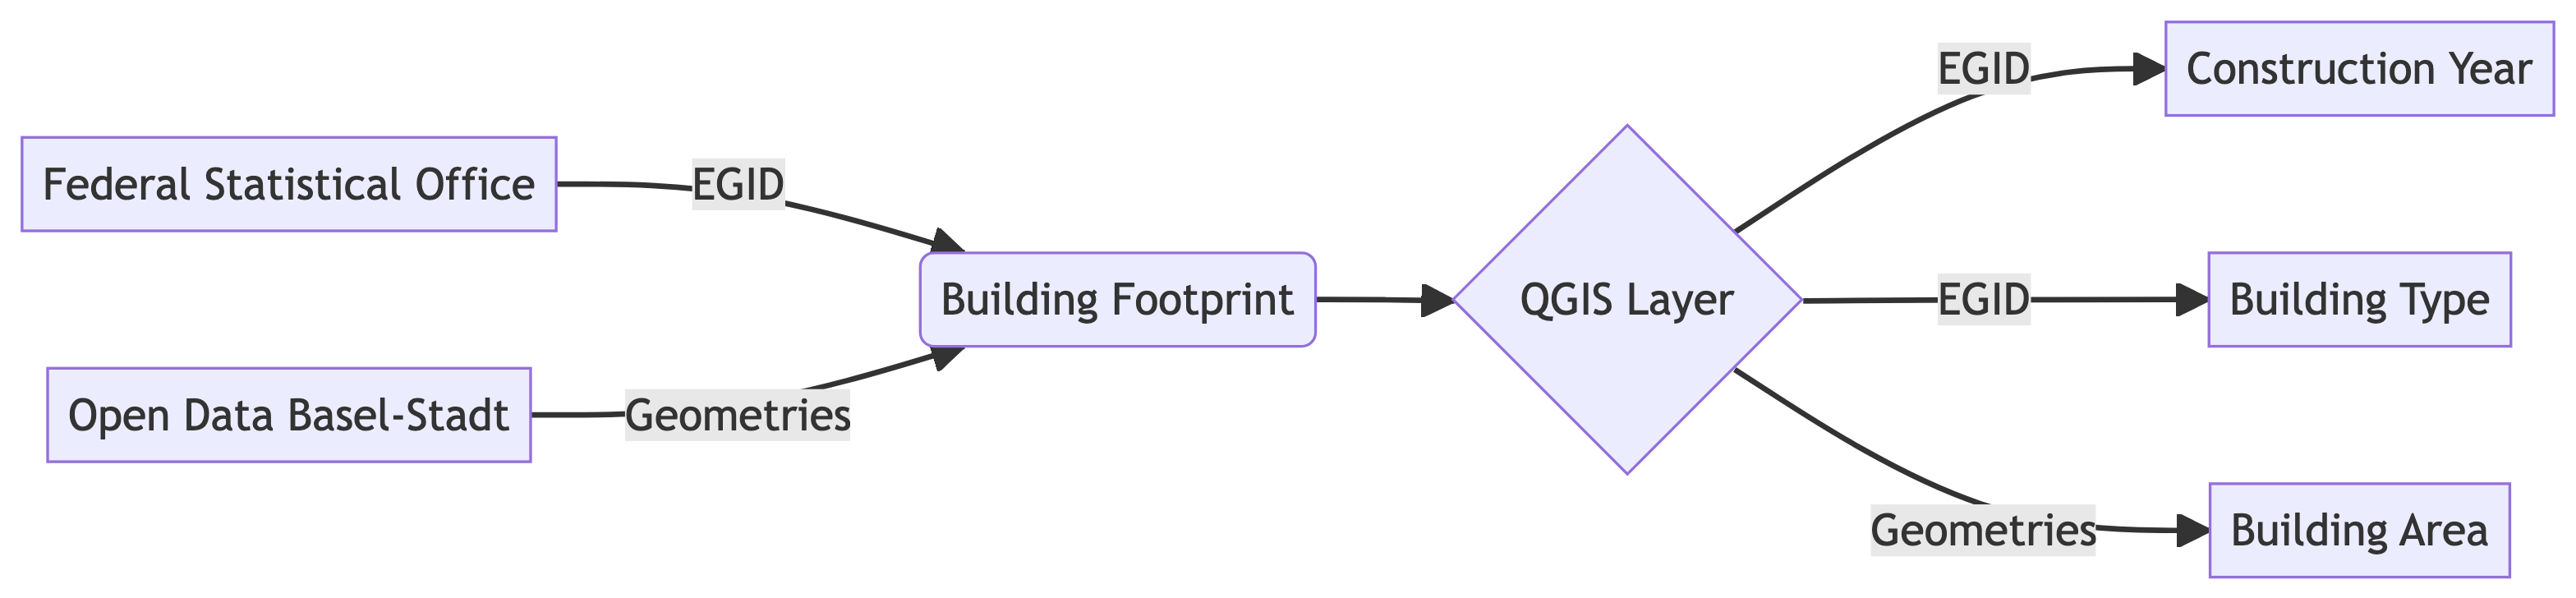
\includegraphics[width=9.76in,height=2.27in]{palimpsest-bs_files/figure-latex/mermaid-figure-1.png}

\textsubscript{Source:
\href{https://mtwente.github.io/palimpsest-bs/palimpsest-bs.qmd.html}{Article
Notebook}}

\section{Feldbergstrasse: City-Wide
Implementation?}\label{feldbergstrasse-city-wide-implementation}

\ldots{}

\subsection{GIS Analysis}\label{gis-analysis}

\ldots{}

\section{Aeschenvorstadt 68: Last Man
Standing}\label{aeschenvorstadt-68-last-man-standing}

\ldots{}

\subsection{Current Situation}\label{current-situation}

\ldots{}

\section{Nauentunnel/Heuwaage-Viadukt}\label{nauentunnelheuwaage-viadukt}

Life after the Correction Plans

\phantomsection\label{refs}
\begin{CSLReferences}{1}{0}
\bibitem[\citeproctext]{ref-bernoulli_neuer_1933}
Bernoulli, Hans, and A. Schuhmacher. 1933. {``Ein Neuer {Plan} Für Die
{Altstadt} von {Basel},''} November.
\url{https://doi.org/10.5169/SEALS-86439}.

\bibitem[\citeproctext]{ref-brandenberger_baumgartnerhauser_2023}
Brandenberger, Rebekka, Ulrike Zophoniasson, and Marco Zünd, eds. 2023.
\emph{Die {Baumgartnerhäuser}: {Basel} 1926-1938}. De Gruyter.
\url{https://doi.org/10.1515/9783035626940}.

\bibitem[\citeproctext]{ref-brunner_bauliche_1999}
Brunner, Mirjam. 1999. {``Die Bauliche {Entwicklung} Der {Stadt}
{Basel}.''} In \emph{Die {Basler} {Strassennamen}}, edited by André
Salvisberg, 31--65. Basel: Christoph Merian Verlag.

\bibitem[\citeproctext]{ref-buchdruckerei_vsk_basel_1949}
Buchdruckerei VSK. 1949. {``Basel Wächst, {Korrektionsplan} {Ja}.''}
\url{https://www.recherche-plakatsammlungbasel.ch/objects/35580}.

\bibitem[\citeproctext]{ref-burckhardt_achtung_2019}
Burckhardt, Lucius, Max Frisch, and Markus Kutter. 2019. \emph{Achtung:
Die {Schweiz} - {Der} {Urtext} von {Lucius} {Burckhardt} Über Die {Idee}
Einer Neuen {Stadt}: {Die} {Geschichte} Eines {Buches} von {Lucius}
{Burckhardt}, {Max} {Frisch} \& {Markus} {Kutter}}. Edited by Markus
Ritter and Martin Schmitz. 1. Auflage. Berlin: Martin Schmitz Verlag.

\bibitem[\citeproctext]{ref-corboz_territorium_2001}
Corboz, André. 2001a. {``Das {Territorium} Als {Palimpsest}.''} In
\emph{Die {Kunst}, {Stadt} Und {Land} Zum {Sprechen} Zu Bringen},
143--66. DE GRUYTER. \url{https://doi.org/10.1515/9783035602654.143}.

\bibitem[\citeproctext]{ref-corboz_geschichte_2001}
---------. 2001b. {``Die {Geschichte} Des {Städtebaus} Als
{Bedeutungsforschung}.''} In \emph{Die {Kunst}, {Stadt} Und {Land} Zum
{Sprechen} Zu Bringen}, 55--64. DE GRUYTER.
\url{https://doi.org/10.1515/9783035602654.55}.

\bibitem[\citeproctext]{ref-eisinger_stadte_2004}
Eisinger, Angelus. 2004. \emph{Städte Bauen: {Städtebau} Und
{Stadtentwicklung} in Der {Schweiz} 1940-1970}. Zürich: gta Verlag.

\bibitem[\citeproctext]{ref-eisinger_stadt_2005}
---------. 2005. \emph{Die {Stadt} Der {Architekten}: {Anatomie} Einer
{Selbstdemontage}}. Bauwelt {Fundamente} 131. Gütersloh/Berlin:
Bauverlag. \url{https://doi.org/10.1515/9783764376758}.

\bibitem[\citeproctext]{ref-eisinger_zeitgemasse_2016}
Eisinger, Angelus, and Reto Geiser. 2016. {``Zeitgemässe
{Anachronismen}: Die Stadtplanerischen {Schriften} von {Lucius}
{Burckhardt}, {Markus} {Kutter} Und {Max} {Frisch} Unter Aktuellen
{Vorzeichen} Gesichtet.''} In \emph{Achtung: Die {Schriften}: {Wir}
Selber Bauen Unsre {Stadt}, {Achtung}: Die {Schweiz}, {Die} Neue
{Stadt}}, 13--24. Zürich: Triest.

\bibitem[\citeproctext]{ref-es_atlas_2014}
Es, Evelien van, and Enrico Chapel, eds. 2014. \emph{Atlas of the
Functional City: {CIAM} 4 and Comparative Urban Analysis}. Bussum, the
Netherlands: THOTH Publishers.

\bibitem[\citeproctext]{ref-fingerhuth_bauten_1988}
Fingerhuth, Carl, and Basel-Stadt, eds. 1988. \emph{Bauten Für {Basel}:
1979 - 1987}. Basel: Wepf.

\bibitem[\citeproctext]{ref-gerber_morphologie_2021}
Gerber, Andri, Regula Iseli, Stefan Kurath, and Urs Primas, eds. 2021.
\emph{Morphologie von {Stadtlandschaften}: {Geschichte}, {Analyse},
{Entwurf}}. Berlin: Reimer.

\bibitem[\citeproctext]{ref-gregory_routledge_2018}
Gregory, Ian, Don DeBats, and Don Lafreniere, eds. 2018. \emph{The
{Routledge} {Companion} to {Spatial} {History}}. 1st ed. Milton Park,
Abingdon, Oxon; New York, NY: Routledge, 2018.: Routledge.
\url{https://doi.org/10.4324/9781315099781}.

\bibitem[\citeproctext]{ref-hagmann_kleinbasels_2022}
Hagmann, Daniel, and Tilo Richter. 2022. {``Kleinbasels {Rückgrat}:
{Die} {Clarastrasse} Und Ihre {Umgebung}.''} In \emph{Basel Ungebaut},
edited by Tilo Richter and Christoph Merian Stiftung, 113--28. Basel:
Christoph Merian Verlag.

\bibitem[\citeproctext]{ref-hoflinger_altes_1954}
Höflinger, Jakob. 1954. \emph{Altes {Basel} Und {Neues} {Basel}}. Basel:
Verlag Athena.

\bibitem[\citeproctext]{ref-huber_architekturfuhrer_2014}
Huber, Dorothee. 2014. \emph{Architekturführer {Basel}: Die
{Baugeschichte} Der {Stadt} Und Ihrer {Umgebung}}. Überarb. Aufl. von
1993. Eine {Publikation} Der {Christoph} {Merian} {Stiftung}. Basel:
Christoph-Merian-Verlag.

\bibitem[\citeproctext]{ref-kaufmann_lebendige_1954}
Kaufmann, Rudolf. 1954. {``Die Lebendige {Stadt}.''} In \emph{Altes
{Basel} Und {Neues} {Basel}}, 9--15. Basel: Verlag Athena.

\bibitem[\citeproctext]{ref-kreis_goldene_2000}
Kreis, Georg. 2000. {``Goldene {Jahre} Mit Irritierenden
{Erfahrungen}.''} In \emph{Basel -- {Geschichte} Einer Städtischen
{Gesellschaft}}, 268--312. Basel: Christoph Merian Verlag.

\bibitem[\citeproctext]{ref-lenherr_fortwahrendes_nodate}
Lenherr, Barbara. n.d. {``Fortwährendes {Seilziehen}: {Die} {Heuwaage}
Als Neuralgischer {Stadtort}.''} In \emph{Basel Ungebaut}, edited by
Tilo Richter and Christoph Merian Stiftung, 85--100. Basel: Christoph
Merian Verlag. Accessed January 23, 2024.
\url{https://basel.swisscovery.org/discovery/fulldisplay?docid=alma9972606264305504&context=L&vid=41SLSP_UBS:live&lang=de&search_scope=UBS&adaptor=Local\%20Search\%20Engine&tab=UBS&query=any,contains,lenherr\%20heuwaage&offset=0}.

\bibitem[\citeproctext]{ref-malfroy_morphologische_2018}
Malfroy, Sylvain, and Gianfranco Caniggia. 2018. \emph{Die
Morphologische {Betrachtungsweise} von {Stadt} Und {Territorium}}.
Zweite Auflage. Zürich: Triest Verlag.

\bibitem[\citeproctext]{ref-mohle_profanes_2016}
Möhle, Martin. 2016. {``Profanes Im {Herzen} Der {Stadt}.''} In
\emph{Kantonale {Denkmalpflege} {Basel}-{Stadt}: {Jahresbericht} 2016},
102--5. Basel: Bau- und Verkehrsdepartement des Kantons Basel-Stadt.

\bibitem[\citeproctext]{ref-mohle_stadtplananalyse_2018}
---------. 2018. {``Stadtplananalyse : Eine Historisch-Methodische
{Einführung}.''} \url{https://doi.org/10.5169/SEALS-787417}.

\bibitem[\citeproctext]{ref-redaktion_der_schweizerischen_bauzeitung_kampf_1949}
Redaktion der Schweizerischen Bauzeitung, and Hans Bernoulli. 1949.
{``Der {Kampf} Um Den {Korrektionsplan} Für {Grossbasel},''} December.
\url{https://doi.org/10.5169/SEALS-84161}.

\bibitem[\citeproctext]{ref-russi_basler_2022}
Russi, Ariane. 2022. \emph{Basler {Plätze}: {Visitenkarten} Der
{Stadt}}. Basel: Friedrich Reinhardt Verlag.

\bibitem[\citeproctext]{ref-salvisberg_basler_1999}
Salvisberg, André, ed. 1999. \emph{Die {Basler} {Strassennamen}}. Basel:
Christoph-Merian-Verl.

\bibitem[\citeproctext]{ref-salvisberg_historischer_2010}
---------. 2010. \emph{Historischer {Atlas} Der {Region} {Basel}:
{Geschichte} Der {Grenzen}}. Basel: Christoph Merian Verlag.

\bibitem[\citeproctext]{ref-schachenmann_altstadtsanierung_1973}
Schachenmann, Felix. 1973. {``Altstadtsanierung Und {Cityring}.''} In,
1973:49--58. Basler {Stadtbuch}. Basel: Christoph Merian Verlag.
\url{https://www.baslerstadtbuch.ch/.permalink/stadtbuch/9fe10c2c-8b1b-46fa-b4fa-2a18144dcf2c}.

\bibitem[\citeproctext]{ref-schneider-sliwa_strategien_1998}
Schneider-Sliwa, Rita, Ulrike Zophoniasson-Baierl, and Fritz Schumacher.
1998. {``Strategien Gegen Den Drohenden {Niedergang} Der {Stadt} : Ein
{Streitgespräch} Zwischen Dem {Basler} {Kantonsbaumeister} {Fritz}
{Schumacher} Und Der {Geographieprofessorin} {Rita}
{Schneider}-{Sliwa}.''} \url{https://doi.org/10.5451/UNIBAS-EP34707}.

\bibitem[\citeproctext]{ref-schnell_architekturkrise_2013}
Schnell, Dieter, and Berner Fachhochschule, eds. 2013. \emph{Die
{Architekturkrise} Der 1970er-{Jahre}: Zur {Jahresausstellung}
{Architektur} Der {Berner} {Hochschule} Für {Architektur}, {Holz} Und
{Bau} Im {Frühling} 2013}. Baden: Hier + Jetzt, Verl. für Kultur und
Geschichte.

\bibitem[\citeproctext]{ref-schuhmacher_basler_1933}
Schuhmacher, A. 1933. {``Der {Basler} {Korrektionsplan}.''} \emph{Das
Werk: Architektur Und Kunst} 20 (11): 345--50.
\url{https://doi.org/10.5169/SEALS-86438}.

\bibitem[\citeproctext]{ref-schulz-rehberg_metamorphosen_2022}
Schulz-Rehberg, Rose Marie. 2022. {``Metamorphosen Und {Visionen}:
{Pläne} Und {Projekte} Für Den {Marktplatz}.''} In \emph{Basel
Ungebaut}, edited by Tilo Richter and Christoph Merian Stiftung, 23--41.
Basel: Christoph Merian Verlag.

\bibitem[\citeproctext]{ref-suter_von_1991}
Suter, Rudolf. 1991. \emph{Von Der Alten Zur Neuen {Aeschenvorstadt}}.
Edited by F. Hoffmann-La Roche AG. Editiones {Roches}. Basel: F.
Hoffmann-LaRoche AG.

\bibitem[\citeproctext]{ref-stoecklin_verschwundenes_2018}
\emph{Verschwundenes {Basel}: Historische {Amateuraufnahmen} von
Verschwundenen {Gebäuden} Und {Anlagen} Der {Stadt} {Basel} Zwischen
1950-1970}. 2018. 2. Auflage. Basel: VB-Verlag.

\bibitem[\citeproctext]{ref-vinken_neuen_2005}
Vinken, Gerhard. 2005. {``Die Neuen {Ränder} Der Alten {Stadt}.
{Modernisierung} Und ‹{Altstadt}-{Konstruktion}› Im Gründerzeitlichen
{Basel}.''} In \emph{Stadtformen. {Die} {Architektur} Der {Stadt}
Zwischen {Imagination} Und {Konstruktion}}, edited by Vittorio Magnago
Lampugnani and Matthias Noell, 130--41. Zürich: gta Verlag.

\bibitem[\citeproctext]{ref-wieland_platz_2022}
Wieland, Benjamin. 2022. {``Der {Platz}, Der Keiner Ist -- Oder:
{Holbein} Wurde Übel.''} \emph{Bz}, January.
\url{https://www.bzbasel.ch/basel/basel-stadt/basler-plaetze-der-platz-der-keiner-ist-oder-holbein-wuerde-uebel-ld.2392987}.

\bibitem[\citeproctext]{ref-wittwer_ludwig_1987}
Wittwer, Hans-Jakob. 1987. {``Ludwig {Marings} ‹{Generalplan} Der
{Stadt} {Basel}› von 1857.''} \emph{Basler Stadtbuch} 1987: 159--64.
\url{https://www.baslerstadtbuch.ch/.download/stadtbuch/aa331a19-6ec0-4db6-a68d-29f7a188b00f}.

\bibitem[\citeproctext]{ref-wullschleger_heuwaage-viadukt_1965}
Wullschleger, Max. 1965. {``Der {Heuwaage}-{Viadukt} -- Eine Gute
Städtebauliche {Lösung}.''} In \emph{Basler {Stadtbuch}}, 1965:227--30.
Basel: Christoph Merian Stiftung.
\url{http://www.baslerstadtbuch.ch/stadtbuch/1965/1965_1193.html}.

\bibitem[\citeproctext]{ref-zaugg_stadtentwicklung_2010}
Zaugg, Roland. 2010. {``Stadtentwicklung {Basels} Seit 1860.''} In
\emph{Historischer {Atlas} Der {Region} {Basel}: {Geschichte} Der
{Grenzen}}, edited by André Salvisberg, 160--61. Basel: Christoph Merian
Verlag.

\end{CSLReferences}



\end{document}
